% \documentclass[12pt, twoside]{article}
\usepackage[letterpaper, margin=1in, headsep=0.2in]{geometry}
\setlength{\headheight}{0.6in}
%\usepackage[english]{babel}
\usepackage[utf8]{inputenc}
\usepackage{microtype}
\usepackage{amsmath}
\usepackage{amssymb}
%\usepackage{amsfonts}
\usepackage[nomessages]{fp} %\FPeval{\var-name}{2*sin(pi/6)}
\usepackage{siunitx} %units in math. eg 20\milli\meter
\usepackage{yhmath} % for arcs, overparenth command
\usepackage{tikz} %graphics
\usetikzlibrary{quotes, angles, arrows, arrows.meta}
\usepackage{graphicx} %consider setting \graphicspath{{images/}}
\usepackage{parskip} %no paragraph indent
\usepackage{enumitem}
\usepackage{multicol}
\usepackage{venndiagram}

\usepackage{fancyhdr}
\pagestyle{fancy}
\fancyhf{}
\renewcommand{\headrulewidth}{0pt} % disable the underline of the header
\raggedbottom
\hfuzz=2mm %suppresses overfull box warnings

\usepackage{hyperref}

\fancyhead[LE]{\thepage}
\fancyhead[RO]{\thepage \\ Name: \hspace{4cm} \,\\}
\fancyhead[LO]{BECA / Dr. Huson / Geometry\\*  Unit 1: Segments, length, and area\\* 19 Sept 2022}

\begin{document}

\subsubsection*{1.8 Homework: Area of rectangles, triangles, parallelograms}
\begin{enumerate}
\item Do Now: Find the area of the parallelogram shown with a base $b=5$ and height $h=3$. 
  \begin{multicols}{2}
    Show the calculation by substituting values for base and height in the formula \\[0.5cm]
    $A = \rm{base} \times \rm{height}$ 
      \begin{flushright}
      \begin{tikzpicture}[scale=.635]
        \draw [help lines] (-1,-1) grid (9,6);
        \draw [thick, ->] (-1.2,0) -- (9.4,0) node [below right] {$x$};
        \draw [thick, ->] (0,-1.2)--(0,6.4) node [left] {$y$};
        \draw [<->, thick] (1.5,1)--(1.5,4);
        \draw [-, thick] (2,1)--(7,1)--(8,4)--(3,4)--cycle;
        \node at (4.5,1)[below]{$5$};
        \node at (1.5,2.5)[left]{$3$};
      \end{tikzpicture}
      \end{flushright}
  \end{multicols} 

\item Rectangle $ABCD$ has area $A=21$ and base $AB=7$ but unknown height. Write an equation then solve. Start with this form (for the unknown, use $h$, $x$, or $BC$): \\[0.5cm]
$A = b \times h = 21$
  \begin{flushright}
  \begin{tikzpicture}[scale=1.25]
    \draw [-, thick] (0,0)--(4.5,0)--(4.5,2)--(0,2)--cycle;
    \draw [fill] (0,0) circle [radius=0.05] node[left]{$A$};
    \draw [fill] (4.5,0) circle [radius=0.05] node[right]{$B$};
    \draw [fill] (4.5,2) circle [radius=0.05] node[right]{$C$};
    \draw [fill] (0,2) circle [radius=0.05] node[left]{$D$};
    \node at (5, 1){?};
    \node at (2.25, -0.5){$7$};
    \node at (2.25, 1){$A = 21$};
  \end{tikzpicture}
  \end{flushright}

\item Find the length of the base of a rectangle with area $A=22 \frac{1}{2}$ and height $h=5$, expressed as a fraction. Start with the form (use $b$ or $x$): \\[0.5cm]
$A = b \times h = 22 \frac{1}{2}$
  \begin{flushright}
  \begin{tikzpicture}[scale=1.25]
    \draw [-, thick] (0,0)--(3,0)--(3,3.5)--(0,3.5)--cycle;
    \node at (3.5, 2){5};
    \node at (1.5, -0.5){$?$};
    \node at (1.5, 2){$A = 22 \frac{1}{2}$};
  \end{tikzpicture}
  \end{flushright}

\item The $\triangle DEF$ has an area $A=24$ and base $DE=8$.
  \begin{multicols}{2}
    Find its height, starting with an equation. \\[0.5cm]
    $\displaystyle A = \frac{1}{2} bh = 24$ \vspace{2cm}
      \begin{flushright}
      \begin{tikzpicture}[scale=.635]
        %\draw [help lines] (-1,-1) grid (9,6);
        \draw [thick, ->] (-1.2,0) -- (9.4,0) node [below right] {$x$};
        \draw [thick, ->] (0,-1.2)--(0,6.4) node [left] {$y$};
        \draw [<->, thick] (0.5,1)--(0.5,5);
        \draw [-, thick] (2,1)--(7,1)--(1,5)--cycle;
        \draw [-, dashed] (7,1)--(6,5)--(1,5);
        \draw [fill] (2,1) circle [radius=0.05] node[below] {$D$};
        \draw [fill] (7,1) circle [radius=0.05] node[below] {$E$};
        \draw [fill] (1,5) circle [radius=0.05] node[above right] {$F$};
        \node at (4.5,1)[below]{$8$};
        \node at (0.5,3)[right]{$h$};
      \end{tikzpicture}
      \end{flushright}
  \end{multicols}

\item Find the length of the base of a triangle with area $A=35$ and height $h=10$. Start with the form (use $b$ or $x$): \\[0.5cm]
$A = \frac{1}{2} \times b \times h = 35$
  \begin{flushright}
  \begin{tikzpicture}[scale=1.25]
    \draw [-, thick] (0,0)--(3,0)--(2.5,3.5)--cycle;
    \node at (3.3, 1.5){10};
    \node at (1.5, -0.5){$?$};
    \node at (1.75, 1){$A = 35$};
  \end{tikzpicture}
  \end{flushright}

\item Given circle $O$ with area $A=121 \pi$ square centimeters.
  \begin{multicols}{2}
  \raggedcolumns
  Find the radius of circle, $OP$. Start with the formula\\[0.5cm]
  $A = \pi r^2 = 121 \pi$ \vspace{1.7cm}
    \begin{tikzpicture}[scale=1]
      \draw (0,0) circle[radius=3];
      \draw [thick]
      (0:3) node[right] {$P$}--
      (0,0) node[below] {$O$};
      \draw (1.5,0) node[below] {$?$};
    \end{tikzpicture}
  \end{multicols}

\end{enumerate}
\end{document}